%! TEX root = ../main.tex
\chapter{研究设计}
\section{极端天气的范围定义}\label{sec:def}

在国际气候变化检测和指数专家组(Expert Team on Climate Change Detection and Indices, ETCCDI)研究\citep{alexander2006global}中定义了27个具有代表性的气候指数标准,具体定义见表\ref{tab:ETCCDI}。这些气候指数被分为两大类别,其中包含了16个与气温相关的指数和11个与降水相关的指数。这些指数不仅为科学家们提供了一个量化气候变化的框架,也为政策制定者和保险业提供了评估气候风险的重要工具。高温对于人身险\citep{马姝瑞2014}和农险\citep{梁来存2019气温天气指数保险的费率厘定}有一定的促进作用,但对于财产保险影响并不直观。虽然高温可能会导致一些直接损害,如房屋过热造成的结构问题,但这些损害通常不如极端降水事件那样显著。极端降水事件则可能带来如洪水和暴雨,导致更广泛的财产损失,包括房屋损坏、基础设施破坏等。且极端高温的尾部数据分布较为集中\citep{尹红2019基于},几十年一遇的高温和数年一遇的高温之间温度差异可能只有低个位数摄氏度。鉴于此,本文选择将极端降水作为极端天气事件的代表来进行深入分析。
%https://www.climdex.org/learn/indices/
\begin{longtable}{cccc}
    \caption{ETCCDI指标}\label{tab:ETCCDI}
    \\
    \toprule
    \multicolumn{2}{c}{\textbf{温度类}} & \multicolumn{2}{c}{\textbf{降水类}} \\
    \cmidrule(rl){1-2} \cmidrule(rl){3-4}
    指标     & 描述             & 指标    & 描述             \\
    \midrule
    FD       & 霜冻日数           & Rx1day  & 最大1日降水量        \\
    SU       & 夏日数            & Rx5day  & 最大连续5日降水量      \\
    ID       & 结冰日数           & SPI     & 标准化降水指数        \\
    TR       & 热夜次数           & SPEI    & 标准化降水蒸发指数      \\
    GSL      & 生长季长度          & SDII    & 简单降水强度指数       \\
    TXx      & 日最高温度最大值       & R10mm   & 降水量≥10mm的天数    \\
    TNx      & 日最低温度最大值       & R20mm   & 降水量≥20mm的天数    \\
    TXn      & 日最高温度最小值       & Rnnmm   & 降水量≥nn mm的天数   \\
    TNn      & 日最低温度最小值       & CDD     & 连续无降水天数最大值     \\
    TN10p    & 低于10百分位数的天数百分比 & CWD     & 连续有降水天数最大值     \\
    TX10p    & 低于10百分位数的天数百分比 & R95p    & 高于95百分位数的年总降水量 \\
    TN90p    & 高于90百分位数的天数百分比 & R99p    & 高于99百分位数的年总降水量 \\
    WSDI     & 暖期持续指数         & R95pTOT & R95p对总降水量的贡献   \\
    DTR      & 日温差            & R99pTOT & R99p对总降水量的贡献   \\
    ETR      & 极端温差           & PRCPTOT & 年总降水量          \\
    CDDcoldn & 冷却度日数          &         &                \\
    GDDgrown & 生长度日数          &         &                \\
    HDDheatn & 加热度日数          &         &                \\
    TMge5    & TM ≥ 5°C的天数    &         &                \\
    TMlt5    & TM < 5°C的天数    &         &                \\
    TMge10   & TM ≥ 10°C的天数   &         &                \\
    TMlt10   & TM < 10°C的天数   &         &                \\
    TMm      & 平均温度           &         &                \\
    TXm      & 平均最高温          &         &                \\
    TNm      & 平均最低温          &         &                \\
    TXge30   & TX ≥ 30°C的天数   &         &                \\
    TXge35   & TX ≥ 35°C的天数   &         &                \\
    TXgt50p  & 高于平均气温的天数百分比   &         &                \\
    TNlt2    & TN < 2°C的天数    &         &                \\
    TNltm2   & TN < -2°C的天数   &         &                \\
    TNltm20  & TN < -20°C的天数  &         &                \\
    TXbdTNbd & 连续寒冷日和夜数       &         &                \\
    \bottomrule
\end{longtable}


对于极端降雨强度的定义,国家标准 GB/T 33680-2017《暴雨灾害等级》中将日降水量超过 50mm 定义为暴雨,超过 250mm 定义为特大暴雨。然而,由于不同地区在气候特征和降水模式上存在显著差异,单一的数值标准可能无法全面反映极端降水事件的影响。参考ETCCDI采用分位数来定义极端天气的方法,将日降水量超过95th或99th百分位数的情况定义为极端降水,这种方法能够更好地适应不同地区的降水特征,因此本文选择将极端降水天气定义为20年一遇的降水天气。

而关于极端降雨受灾范围的界定,结合降水数据和保单数据(见\ref{sec:data}),考虑到绝大多数保险标的与距离最近的气象站之间距离大多在50公里以内,平均距离不足30公里,如图\ref{fig:distance},因此本文将距离监测到极端降水的气象站20公里内的区域定义为灾区。而考虑到我国气象站分布间距基本在100公里以内,如图\ref{fig:locations},因此取气象站所覆盖的受灾半径最多为50公里,定义距离监测到极端降水的气象站20-50公里内的区域为近灾区,50公里以上的区域为远灾区。

\begin{figure}[H]
    \begin{minipage}{0.48\linewidth}
        \centering
        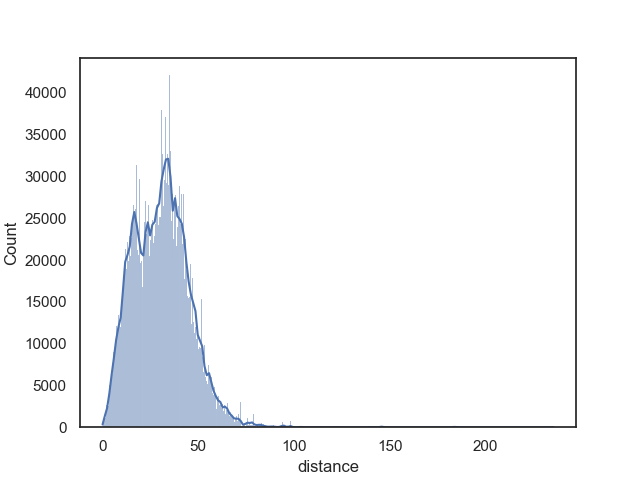
\includegraphics[width=\textwidth]{lib/img/distance.png}
        \caption{原始数据中保险标与最临近气象站的距离分布(千米)}
        \label{fig:distance}
    \end{minipage}
    \begin{minipage}{0.48\linewidth}
        \centering
        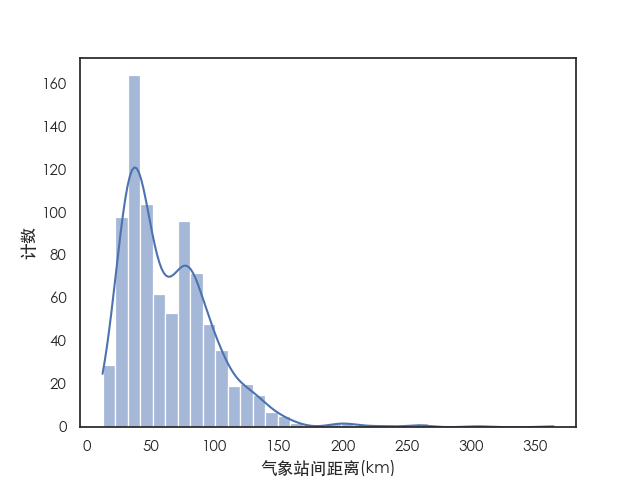
\includegraphics[width=\textwidth]{lib/img/locations_distance.png}
        \caption{原始数据中气象站间距的地理位置分布(千米)}
        \label{fig:locations}
    \end{minipage}
\end{figure}

\section{样本选择与数据清理}\label{sec:data}

本文选取了中国气象局的气象数据和某财产保险公司的承保理赔保险数据作为研究数据。空间范围上,二者均覆盖全国。大多数研究在数据预处理时通常聚类至县市一级行政区划\citep{0Do,杨娜娜2019自然灾害与企业现金持有},得益于GIS技术的发展和普及化,本文对于数据的处理相较于更为精细,直接根据经纬度信息计算距离,不再依赖行政区划的聚类。时间维度上,气象数据时间范围为1954年1月1日至2015年12月31日,保险数据时间范围为1995年1月1日至2019年12月31日,数据清洗时保留1995-2015年数据。最终将1914万条气象数据与610万条保单数据进行了匹配,得到71万条数据用于回归分析。

\begin{figure}[H]
    \centering
    \includegraphics[width=\textwidth]{lib/img/locations.png}
    \caption{原始数据中气象站的地理位置分布}
    \label{fig:location}
\end{figure}

\section{模型设定与变量定义}

极端天气事件是一个外生冲击,在时空上的分布是随机的,因此本文采用了DID回归来估计极端天气事件对家庭财产保险的影响。DID回归的基本思想是通过对照组和实验组的比较,消除了时间不变的个体特征对估计结果的影响,从而更加准确地估计政策的效果。本文设定了一个虚拟的实验组和对照组,实验组为受灾区或近灾区,对照组为未受灾区,通过比较两组在巨灾发生前后的差异来估计极端天气事件对财产保险的影响。

本文采用的被解释变量为家财险保额,反映家庭对财产保险的需求。而解释变量为极端天气事件的虚拟变量,分为两个维度:是否受灾和是否邻近灾区。控制变量包括是否历史投保、保险财产购置价、建筑面积等,以期消除其他因素对家庭财产保险需求的影响。各类变量及其定义如表\ref{tab:var}所示。
\begin{table}[H]
    \caption{变量定义表}\label{tab:var}
    \centering
    \begin{tabular}{@{}cccc@{}}
        \toprule
        变量类别                    & 变量名称         & 变量定义    & 变量解释                \\ \midrule
        被解释变量                   & Coverage     & 保额      & 保险金额                \\ \midrule
        \multirow{3}{*}{主要解释变量} & Disaster     & 灾区      & 是否处于极端降水监测点20公里内    \\ \cmidrule(l){2-4}
                                & Neighbor     & 近灾区     & 是否处于极端降水监测点20-50公里内 \\ \cmidrule(l){2-4}
                                & Post         & 降水发生时间  & 是否在极端降水发生后投保        \\
        \midrule
        \multirow{3}{*}{控制变量}   & Prem\_before & 历史投保    & 保险标的是否有投保记录         \\ \cmidrule(l){2-4}
                                & Price        & 保险财产购置价 & 保险标的资产购置价           \\ \cmidrule(l){2-4}
                                & Area         & 建筑面积    & 保险标的建筑面积            \\ %\cmidrule(l){2-4}
        % & Claim       & 是否理赔    & 该保单是否发生理赔            \\
        \bottomrule
    \end{tabular}
\end{table}


针对假设H\ref{hyp:1}与H\ref{hyp:2}本文的DID模型如下:

\begin{equation}
    \text{Coverage}=\alpha+\beta_1\text{Disaster}+\beta_2\text{Post}+\beta_3\text{Disaster}\times\text{Post}+\beta\text{Controls}+\varepsilon
    \label{eq:DID_1}
\end{equation}

而针对假设H\ref{hyp:3}本文的DID模型如下:

\begin{equation}
    \text{Coverage}=\alpha+\beta_1\text{Neighbor}+\beta_2\text{Post}+\beta_3\text{Neighbor}\times\text{Post}+\beta\text{Controls}+\varepsilon
    \label{eq:DID_2}
\end{equation}
